% Chapter Template

\chapter{LeNet Architecture and  Quantization}\doublespacing % Main chapter title

\label{Chapter2} % Change X to a consecutive number; for referencing this chapter elsewhere, use \ref{ChapterX}

\lhead{Chapter II. \emph{Neural Network Architecture and Quantization}} % 

\section{Introduction}
In the domain of computer vision and image processing, Convolutional Neural Networks (CNNs) have emerged as a powerful tool for image classification tasks. One of the pioneering architectures in this field is LeNet, introduced by Yann LeCun and his colleagues in the late 1980s and early 1990s. LeNet was specifically designed to recognize handwritten digits in the MNIST dataset, a benchmark dataset consisting of 60,000 training images and 10,000 testing images of handwritten digits from 0 to 9. Each image in the dataset is of size 28x28 pixels with a single color channel (grayscale).
\\
The LeNet architecture is structured to efficiently handle the spatial hierarchy of features within an image. It consists of two convolutional layers, each followed by a subsampling (pooling) layer, and two fully connected layers leading to an output layer with 10 neurons, each corresponding to one of the digit classes. The design of LeNet allows it to automatically learn hierarchical features from raw pixel values, significantly improving the accuracy of digit recognition.
\\
\textbf{Architecture Overview:}
\begin{figure}[h]
    \centering
    % \includegraphics[width=\linewidth]{Chapters/Chapter_2/images/lenet.png}
    \includegraphics[width=\linewidth]{../figures/lenet.png}
    \caption{LeNet Architecture}
    % \label{fig:your_label}
\end{figure}

\begin{enumerate}
  \item \textbf{Input Layer:} The input to the network is a 32x32x1 gray scale image.
  \item \textbf{Convolutional Layer 1:} This layer consists of six 5x5 filters (kernels), producing six feature maps of size 28x28.
  \item \textbf{Subsampling (Pooling) Layer 1:} A 2x2 max pooling operation reduces the size of each feature map to 14x14.
  \item \textbf{Convolutional Layer 2:} This layer applies sixteen 5x5 filters to the pooled output, resulting in sixteen 8x8 feature maps.
  \item \textbf{Subsampling (Pooling) Layer 2:} Another 2x2 max pooling operation further reduces the feature maps to 5x5.
  \item \textbf{Fully Connected Layer 1:} The flattened output from the second pooling layer (16 x 5 x 5 = 400 units) is fed into a fully connected layer with 120 units.
  \item \textbf{Fully Connected Layer 2:} This layer consists of 84 units, further refining the learned features.
  \item \textbf{Output Layer:} Finally, the network outputs a probability distribution over the 10 digit classes using a soft max activation function.
  % \item Another entry in the list
\end{enumerate}
LeNet's simple yet effective architecture has laid the foundation for more complex CNNs and has been instrumental in advancing the field of deep learning. Its ability to achieve high accuracy on the MNIST dataset with relatively few parameters makes it an ideal starting point for exploring CNNs in the context of handwritten digit recognition.


\section{Convolution Operation}
The convolution operation is a mathematical process used to extract features from an input image. It involves sliding a filter (also known as a kernel) across the input image and computing the dot product between the filter and a region of the image. The result of this operation is a feature map that highlights various aspects of the input image, such as edges, textures, and patterns.
\\
Mathematically, the convolution operation for a single output pixel can be expressed as:

\begin{equation}
(I * K)(i, j) = \sum_{m} \sum_{n} I(i + m, j + n) \cdot K(m, n)
\end{equation}

where:
\begin{itemize}
  \item $I$ is the input image,
  \item $K$ is the kernel,
  \item $i, j$ are the coordinates of the output feature map,
  \item $m, n$ are the coordinates within the kernel.
\end{itemize}

The  pseudocode for the convolution operation:

\begin{lstlisting}[language=Python, caption=Pseudocode for 2D Convolution Operation]
function Convolution2D(input, kernel):
    input_height, input_width = dimensions of input
    kernel_height, kernel_width = dimensions of kernel
    output_height = input_height - kernel_height + 1
    output_width = input_width - kernel_width + 1
    
    # initialize output as zeros with dimensions (output_height, output_width)
    
    for i = 0 to output_height - 1:
        for j = 0 to output_width - 1:
            sum = 0
            for m = 0 to kernel_height - 1:
                for n = 0 to kernel_width - 1:
                    sum += input[i+m][j+n] * kernel[m][n]
            output[i][j] = sum
    
    return output
\end{lstlisting}

\section{Pooling Operation}
Pooling is a down-sampling operation that reduces the spatial dimensions of the feature map, thereby reducing the number of parameters and computation in the network. It also helps in making the detection of features invariant to small translations.\\
The max pooling operation can be expressed as:

\begin{equation}
Y(i, j) = \max_{0 \leq m < p} \max_{0 \leq n < q} X(i \cdot s + m, j \cdot s + n)
\end{equation}

where:
\begin{itemize}
  \item $X$ is the input feature map,
  \item $Y$ is the output feature map after max pooling,
  \item $i, j$ are the coordinates of the output feature map,
  \item $p, q$ are the height and width of the pooling window,
  \item $s$ is the stride of the pooling operation,
  \item $m, n$ are the coordinates within the pooling window.
\end{itemize}

\section{Non Linear Activation}
Non-linear activation functions introduce non-linearity into the neural network, allowing it to learn complex patterns in the data. Without non-linear activation functions, the network would behave like a linear model, regardless of the number of layers, limiting its ability to solve complex tasks. Here are some commonly used non-linear activation functions
\begin{enumerate}
    \item \textbf{Sigmoid Function:} The sigmoid activation function maps the input values to a range between 0 and 1. It is often used in the output layer for binary classification problems.
    \begin{equation}
        \sigma(x) = \frac{1}{1 + e^{-x}}
    \end{equation}
    \item \textbf{Rectified Linear Unit (ReLU) Function:} The ReLU activation function is widely used in deep learning models due to its simplicity and effectiveness. It maps the input to zero if it is negative and leaves it unchanged if it is positive.
    \begin{equation}
\text{ReLU}(x) = \max(0, x)
\end{equation}

    \item \textbf{Leaky ReLU Function:} Leaky ReLU is a variant of ReLU that allows a small, non-zero gradient when the input is negative. This helps to avoid the "dying ReLU" problem where neurons get stuck during training.
    \begin{equation}
\text{Leaky ReLU}(x) = \begin{cases}
x & \text{if } x > 0 \\
\alpha x & \text{if } x \leq 0
\end{cases}
\end{equation}

\end{enumerate}

\section{Model Training using Posit Data Type}
\subsection{Posit number system}
The Posit number system, a Type-III universal number representation (Unum), is characterized by two primary parameters: the word size (n) and the exponent field size (es). Unlike conventional floating-point numbers (float), Posit features a distinct regime field encoding scheme based on the run-length method, which enables a more optimal trade-off between dynamic range and numerical precision. This unique encoding approach allows Posit to exhibit improved performance in terms of both range and precision, making it a promising alternative to traditional floating-point representations.\\
\begin{figure}[h]
    \centering
    % \includegraphics[width=\linewidth]{Chapters/Chapter_2/images/posit.png}
    \includegraphics[width=\linewidth]{../figures/posit.png}
    \caption{General posit format }
    % \label{fig:your_label}
\end{figure}
As illustrated in Figure 2.2, a posit number, denoted as (n, es), comprises four distinct components: a \textbf{sign} bit, \textbf{regime} field, \textbf{exponent} field, and \textbf{mantissa} field. The regime field value is decoded by interpreting consecutive sequences of '1's followed by a '0' as k-1 and consecutive sequences of '0's followed by a '1' as -k, where k represents the number of consecutive bits. The value of posit number p(binary code) is given by:
\begin{equation}
\left\{
\begin{array}{ll}
0, & p = 0, \\
\pm\infty, & p = -2^{n-1}, \\
\text{sign}(p) \times useed^k \times 2^e \times f, & \text{all other } p.
\end{array}
\right.
\end{equation}
\subsection{Models Trained using Posit Data Type}
To investigate the impact of employing the Posit data type for storing the output of convolutional layers, a modification was introduced in the training phase of the LeNet architecture, wherein the output of each convolutional stage was stored in the Posit format. This allowed for an exploration of the effects of Posit-based storage on the accuracy of the convolutional neural network (CNN). The resulting accuracy metrics, presented in the following table, provide insight into the efficacy of utilizing Posit data type in this context.\\
\begin{table}[h]
    \centering
    \begin{tabularx}{1.1\textwidth}{|c|X|X|X|X|X|X|}
        \hline
        \textbf{Sr.No} & \textbf{Model} & \textbf{Dataset}  & \textbf{Datatype for computation} & \textbf{Datatype for storage} & \textbf{Training Accuracy} & \textbf{Testing Accuracy} \\
        \hline
        1 &\multirow{4}{*}{LeNet-5}  & \multirow{4}{6em}{MNIST Handwritten Digit}  & 32 bit float  & 32 bit float  & 98.6\% & 98.27\% \\\cline{4 - 7}
        
        2 &  &   & 16 bit float  & 16 bit float  & 97.93\% & 97.23\% \\\cline{4 - 7}
        
        3 &  &   & 32 bit float  & 8 bit posit  & 88\% & 89\% \\\cline{4 - 7}
        
        4 &  &    & 16 bit float  & 8 bit posit  & 88.7\% & 89.37\% \\\hline
   
    \end{tabularx}
    \caption{Impact of Posit Storage on the Accuracy of LeNet Model}
    \label{tab:posti_comparison}
\end{table}\\
The incorporation of Posit-based storage resulted in an accuracy degradation of 8-9\% relative to the baseline architecture, which was found to be more pronounced than expected . Consequently, a comprehensive examination of alternative approaches led to the selection of the Post-Training Quantization (PTQ) method, as implemented in the PyTorch framework, to optimize the quantization process and minimize the accuracy loss. 
\section{Post Training Static Quantization}
Post Training Static Quantization (PTQ) is a technique used in PyTorch to optimize the inference performance of neural networks by converting the model's weights and activations from floating-point precision (usually 32-bit) to integer precision (usually 8-bit). This conversion results in faster computation and reduced memory footprint, making it particularly useful for deployment on edge devices and resource-constrained environments.
\\
PyTorch's PTQ workflow involves the following key steps:
\begin{enumerate}
    \item \textbf{Preparation:}  Modify the model to support quantization by inserting quantization and dequantization nodes.
    \item \textbf{Calibration:} Collect statistics on the distributions of weights and activations by running inference with representative calibration data. The prepared model is run on a set of representative data to collect the necessary statistics (e.g., min and max values) for each layer's activations and weights. This step is crucial for determining the scaling factors and zero points used in quantization.
    \item \textbf{Conversion:} Convert the floating-point model to a quantized model using the collected statistics.After calibration, the model is converted to its quantized form. This step replaces the floating-point weights and activations with their quantized counterparts based on the collected statistics.
\end{enumerate}

Here is a complete example of applying PTQ to a PyTorch model:\\
\begin{lstlisting}[language=Python, caption=PyTorch Post Training Static Quantization]
import torch
import torch.quantization

# Define or load your model
model = MyModel()

# Set the model to evaluation mode
model.eval()

# Specify the quantization configuration
model.qconfig = torch.ao.quantization.default_qconfig

# Prepare the model for static quantization
torch.quantization.prepare(model, inplace=True)

# Calibrate the model with representative data
calibration_data = [...]  # Your calibration dataset
with torch.no_grad():
    for input in calibration_data:
        model(input)

# Convert the model to a quantized version
torch.quantization.convert(model, inplace=True)

# The model is now quantized and ready for inference
\end{lstlisting}
% The resulting accuracy metrics, after using PTQ technique for quantizing the model is given below.
The resulting accuracy metrics, yielded by the employment of PTQ techniques for the quantization and precision scaling of the trained model, are presented in the following table
\begin{table}[h]
    \centering
    \begin{tabularx}{1.1\textwidth}{|c|X|X|X|X|X|X|}
        \hline
        \textbf{Sr.No} & \textbf{Model} & \textbf{Dataset}  & \textbf{Datatype for computation} & \textbf{Datatype for storage} & \textbf{Training Accuracy} & \textbf{Testing Accuracy} \\
        \hline
        1 & \multirow{2}{*}{LeNet-5}  & MNIST Handwritten Digit  & 32 bit float  & 32 bit float  & 98.6\% & 98.27\% \\\cline{4 - 7}
        
        2 &  &   & 32 bit float  & 8 bit UINT  & - & 98.01\% \\\hline

   
    \end{tabularx}
    \caption{Impact of PTQ technique on the Accuracy of LeNet Model}
    \label{tab:PTQ_comparison}
\end{table}\\
% From the above observation, we can see that there is no significant drop in testing accuracy. Hence we chose this method of quantization to test on hardware. 
An examination of the table reveals that the testing accuracy remains relatively invariant, exhibiting no significant degradation, thereby indicating the efficacy of the employed quantization method in maintaining the model's performance. Consequently, this quantization technique was selected for implementation on the hardware platform, as it demonstrates a satisfactory tradeoff between precision and computational efficiency.
% \lipsum[1] \citep{li-1984}.

% Nam dui ligula, fringilla a, euismod sodales, sollicitudin vel, wisi. Morbi auctor lorem
% non justo. Nam lacus libero, pretium at, lobortis vitae, ultricies et, tellus. Donec
% aliquet, tortor sed accumsan bibendum, erat ligula aliquet magna, vitae ornare odio
% metus a mi \citep{li-1984, WHO-2018}.

% Here is Figure \ref{fig:figure2_1}.

% \begin{figure}[ht]
    \centering
    
\includegraphics[width=0.3\textwidth]{Chapters/Chapter_2/figures/image1.png}
    \caption{Plot with a single image (Image by pencil parker from Pixabay)}
    \label{fig:figure2_1}
\end{figure}

% \lipsum[2]

% \begin{figure}[ht]
\centering
\begin{tabular}{cc}

\includegraphics[width=0.3\textwidth]{Chapters/Chapter_2/figures/image1.png} & 
\includegraphics[width=0.3\textwidth]{Chapters/Chapter_2/figures/image1.png} \\
(a) First Sub-caption. & (b) Second sub-caption. \\
\end{tabular}
\caption{Plot with two images in one row}
\label{fig: figure2_2}
\end{figure}

% \lipsum[2]

% \begin{figure}[ht]
\centering
\begin{tabular}{ccc}

\includegraphics[width=0.3\textwidth]{Chapters/Chapter_2/figures/image1.png} & 
\includegraphics[width=0.3\textwidth]{Chapters/Chapter_2/figures/image2.png} & \\
(a) Sub-caption 1 & (b) Sub-caption 2 & \\
\multicolumn{3}{c}{
\includegraphics[width=0.3\textwidth]{Chapters/Chapter_2/figures/image1.png}} \\
\multicolumn{3}{c}{(c) Sub-caption 3} \\
\end{tabular}
\caption{Plot with three images}
\label{fig:figure2_3}
\end{figure}

% \lipsum[2]

% \begin{figure}[htbp] 
\centering
  \begin{tabular}{c c}
    
\includegraphics[width=65mm, height = 55mm]{Chapters/Chapter_2/figures/image1.png}  &    
\includegraphics[width=65mm, height = 55mm]{Chapters/Chapter_2/figures/image1.png} \\
    \vspace{1mm}
    (a) Sub-caption 1 & (b) Sub-caption 2 \\
    
    \vspace{1mm}
    
    
\includegraphics[width=65mm, height = 55mm]{Chapters/Chapter_2/figures/image1.png}
     &
    
\includegraphics[width=65mm, height = 55mm]{Chapters/Chapter_2/figures/image1.png}\\
    \vspace{1mm}
    (c) Sub-caption 3 & (d) Sub-caption 4 \\
    
   
  
  \end{tabular}
 \caption{Plot with two by two image grid.
}
  \label{fig:image2_4}
\end{figure}

% \lipsum[1-2]
% Here is Table \ref{tab: table2_1}.
% \begin{table}[!ht]
  \centering
  \caption{Various empirical study details.}
  \resizebox{\textwidth}{!}{%
    \begin{tabular}{llllll}
    
    \toprule
    \textbf{\makecell[l]{Authors\\ and\\ Country}} & \textbf{\makecell[l]{Type \\ (Number of Sites)}} & \textbf{\makecell[l]{Study\\ Type}} & \textbf{\makecell[l]{Sample\\ Size}} & \textbf{Variable used} & \textbf{\makecell[l]{Model/\\method\\ used}} \\ \midrule

    \makecell[l]{Author 1,\\Canada} & \makecell[l]{School zones\\ (34)} &  \makecell[l]{V}  &  \makecell[l]{567} & \makecell[l]{Variable 1, variable 2,\\ variable 3, variable 4,\\ and variable 5} &   
    \makecell[l]{Linear Regression} \\ \midrule


    \makecell[l]{Author 2,\\France} & \makecell[l]{Mid-block section\\ (4)} &  \makecell[l]{Q}  &  \makecell[l]{120} & \makecell[l]{Variable 1, variable 2,\\ variable 3, variable 4,\\ and variable 5} &   
    \makecell[l]{Survival analysis} \\ \midrule


    \makecell[l]{Author 3,\\Japan} & \makecell[l]{Mid-block section\\ (4)} &  \makecell[l]{O}  &  \makecell[l]{1130} & \makecell[l]{Variable 1, variable 2,\\ variable 3, variable 4,\\ and variable 5} &   
    \makecell[l]{Soft computing} \\ \midrule
    

    \makecell[l]{Author 4,\\Australia} & \makecell[l]{Signalized crosswalk\\ (4)} &  \makecell[l]{E}  &  \makecell[l]{567} & \makecell[l]{Variable 1, variable 2,\\ variable 3, and variable 4} &   
    \makecell[l]{Descriptive statistics} \\
    
    \bottomrule

  
    
    \end{tabular}
    }
{\scriptsize
\begin{minipage}{0.8\textwidth}
    \begin{flushleft}
    \vspace{0.2cm}
        {\scriptsize \textbf{Note:} E: Experimental, O: Observational survey, Q: Questionnaire survey, V: Video graphic survey.}
    \end{flushleft}
\end{minipage}
}
  \label{tab: table2_1}%
\end{table}%



% \section{Research Gaps}
% \lipsum[1-4]



% \section{Summary}
% \lipsum[2]






